Komprimeringsalgoritmen "Huffman coding", er udviklet af David A. Huffman. Huffman udviklede algoritmen, mens han var Ph.D studerende på MIT. I 1952 udgav han dokumentet "A Method for the Construction of Minimum-Redundancy Codes"\cite{A_Method_for}. Her beskrev Huffman, hvordan hans komprimerings algoritme fungerede. Hvad han havde udviklet, var en 'lossless' (tabsfri) komprimerings metode, hvilket betyder, at der ikke vil være noget tab af information ved at komprimere. Komprimeringsmetoden er beregnet til binære systemer, og formålet med algoritmen er at få en given datamængde til at benytte et minimalt antal bit. 

For så at kunne få de orginale data tilbage fra den komprimerede form, kræver det selvfølgelig, at man har en form for ordbog, der beskriver hvilke tegn, der hører sammen med hvilke bits.

For at Huffman coding effektivt kan fungere, skal algoritmen have adgang til hele datamængden, for at kunne analysere hyppigheden af forskellige tegn. Dette betyder at algoritmen skal løbe i gennem datamængden to gange. Første gang, for at indsamle statistik, og anden gang for så at foretage den reelle komprimering. En eksempel på en algoritme der ikke har den ulempe er komprimeringsmetoden "Lempel-Ziv-Welch".


\subsubsection{Generering af Huffman træ}
Huffman algoritmen kigger på frekvensen af tegn, og giver så de hyppigste tegn, den korteste binære kode. For at finde frem til de binære koder til hver tegn, laver man et Huffman træ. Træet gør, at den binære kode til et tegn, aldrig vil være starten på koden til et andet tegn. Træet laves ved først at tælle hyppigheden af de forskellige tegn brugt i datamængden der skal komprimeres, og derefter tage de to tegn med lavest frekvens, og lave et nyt punkt, med frekvensen af det første og andet tegn lagt sammen. Dette gøres så indtil der kun er et punkt tilbage. Dette punkt er så toppen af træet. For så at finde frem til den binære kode for hvert tegn, starter man i toppen af træet, og tilføjer 0 eller 1, hvis man gå til henholdsvis venstre eller højre.
\\
\\
Hvis vi kigger på sætningen "dette er et eksempel", viser tabel \ref{tab:huffmantable_new} de forskellige tegn brugt i sætningen, sorteret efter hyppighed. Her tager vi så de to tegn med lavest frekvens (fx D og K), og laver et nyt punkt, med frekvensen af det første og andet tegn lagt sammen. Dette nye punkt, sættes så ind i listen, i stedet for de to tegn. Herefter laves der igen et punkt, med de to tegn/punkter med lavest frekvens, og dette gøres til der kun er et punkt tilbage. Det endelige resultat, bliver så Huffman træet, figur \ref{fig:huffmantree}. 



\begin{figure}[hba]
\centering
\begin{tabular}{|c|c|}
\hline
\cellcolor{ForestGreen}\color{white}{\textbf{Tegn}} &
\cellcolor{ForestGreen}\color{white}{\textbf{Frekvens}} \\ 
\hline 
E & 7 \\ 
\hline 
SPACE & 3 \\ 
\hline 
T & 3 \\ 
\hline 
R & 1 \\ 
\hline 
P & 1 \\ 
\hline 
S & 1 \\ 
\hline 
M & 1 \\ 
\hline 
L & 1 \\ 
\hline 
D & 1 \\ 
\hline 
K & 1 \\ 
\hline 
\end{tabular} 
\caption{Frekvens for tegn i sætningen ''dette er et eksempel''}
\label{tab:huffmantable_new}
\end{figure}

\begin{figure}[H]
\centering
%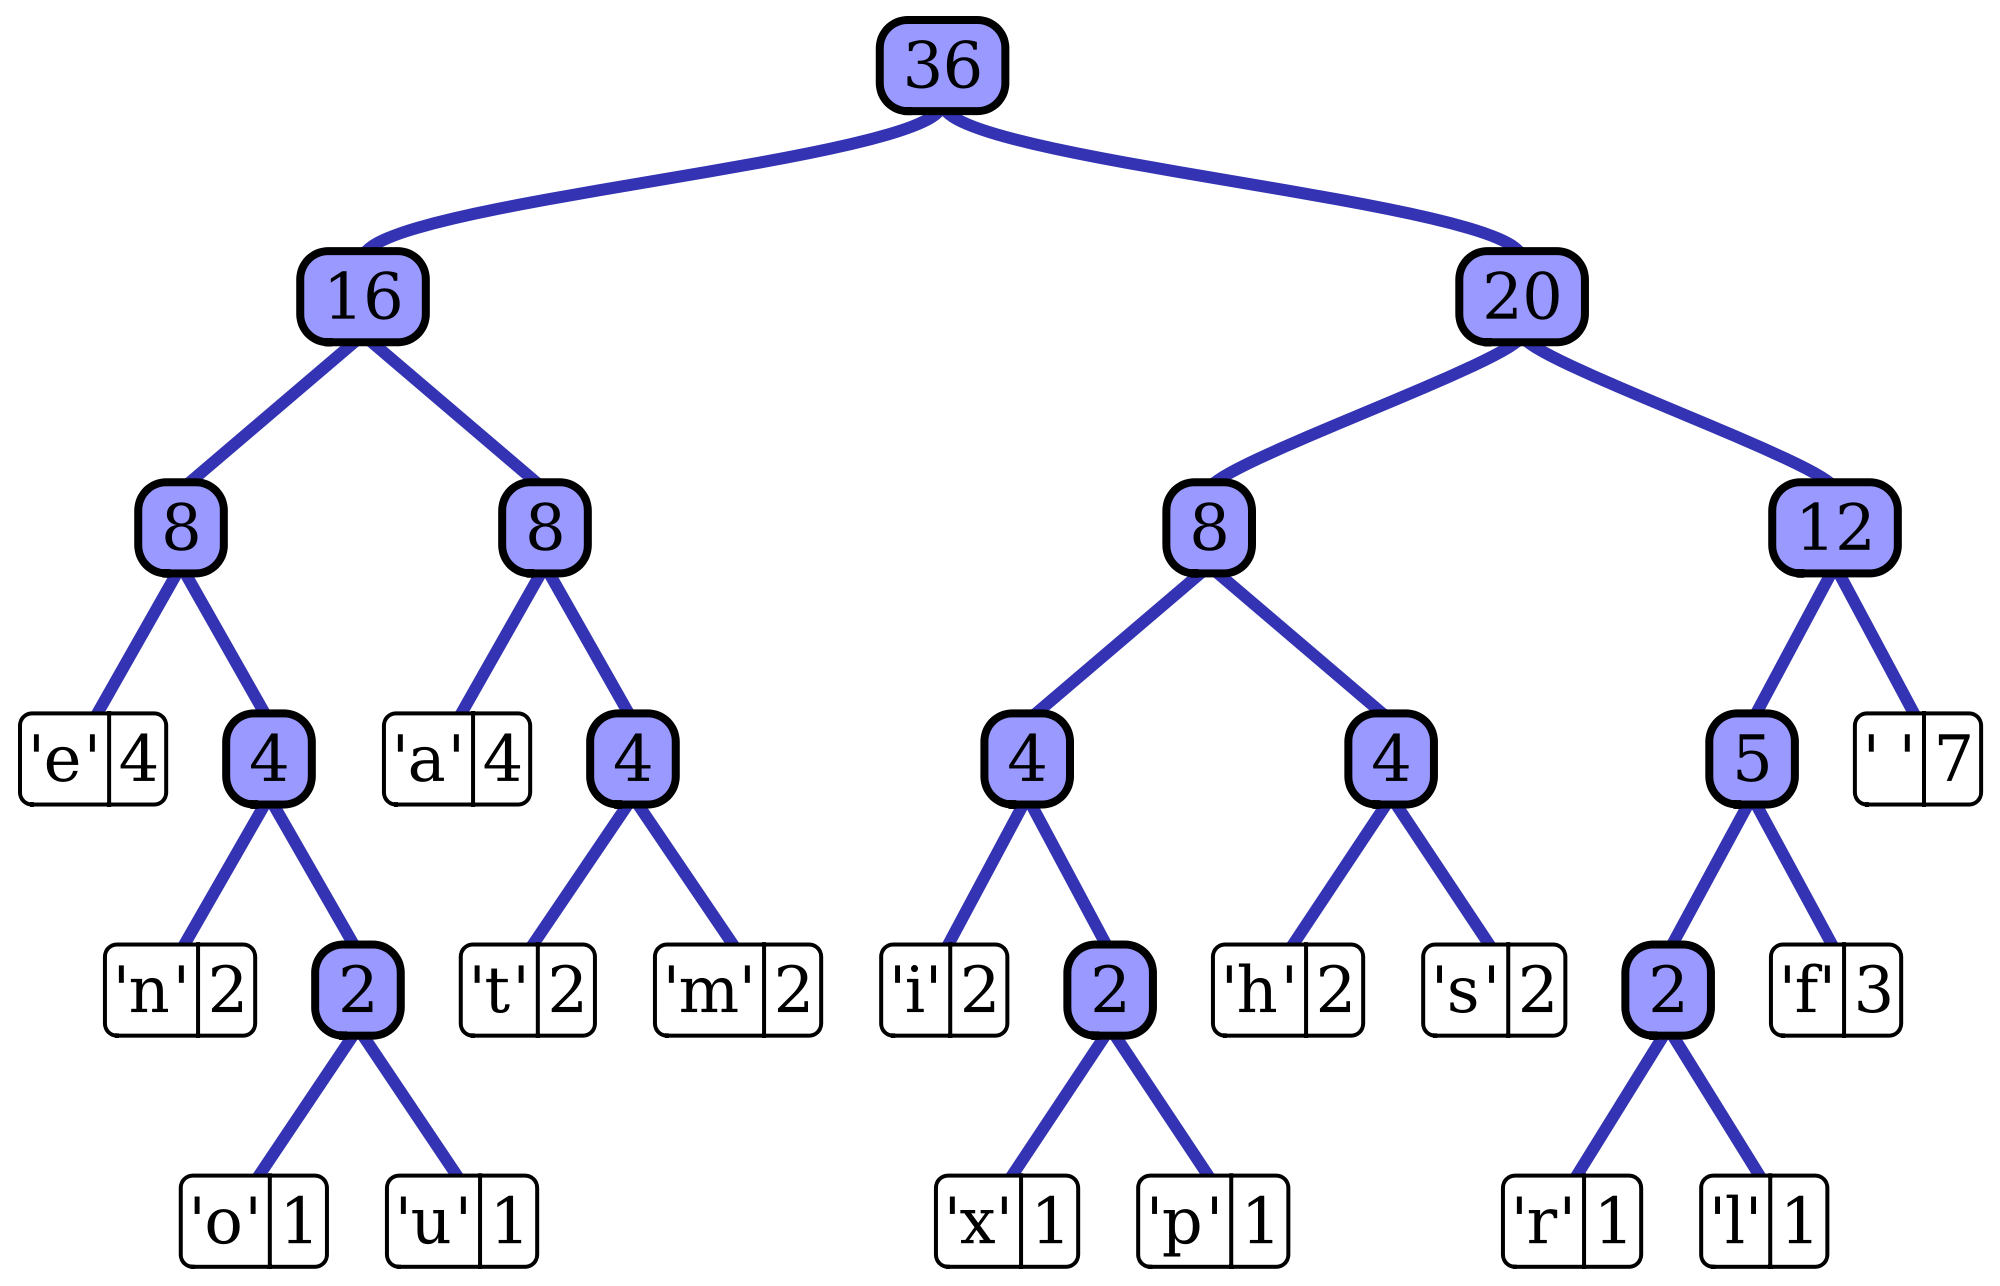
\includegraphics[width=\linewidth]{Billeder/Huffman_tree_2.png}
%

%

%

%
%
%

\enlargethispage{100cm}
% Start of code
% \begin{tikzpicture}[anchor=mid,>=latex',line join=bevel, scale=0.5]
\begin{tikzpicture}[>=latex',line join=bevel, scale=0.8]
  \pgfsetlinewidth{1bp}
%%
\pgfsetcolor{black}
  % Edge: ML -> L
  \draw [->] (271bp,85.689bp) .. controls (271bp,77.317bp) and (271bp,66.99bp)  .. (271bp,47.016bp);
  \definecolor{strokecol}{rgb}{0.0,0.0,0.0};
  \pgfsetstrokecolor{strokecol}
  \draw (274.5bp,64bp) node {1};
  % Edge: 2 -> S
  \draw [->] (127bp,85.689bp) .. controls (127bp,77.317bp) and (127bp,66.99bp)  .. (127bp,47.016bp);
  \draw (130.5bp,64bp) node {1};
  % Edge: 20 -> E
  \draw [->] (115.2bp,388.3bp) .. controls (112.76bp,381.27bp) and (109.84bp,372.85bp)  .. (103.66bp,355.07bp);
  \draw (116.5bp,372bp) node {0};
  % Edge: DK -> K
  \draw [->] (356.54bp,88.329bp) .. controls (365.3bp,78.844bp) and (377bp,66.163bp)  .. (394.43bp,47.282bp);
  \draw (388.5bp,64bp) node {1};
  % Edge: DK -> D
  \draw [->] (343bp,85.689bp) .. controls (343bp,77.317bp) and (343bp,66.99bp)  .. (343bp,47.016bp);
  \draw (346.5bp,64bp) node {0};
  % Edge: 2 -> P
  \draw [->] (113.46bp,88.329bp) .. controls (104.7bp,78.844bp) and (92.997bp,66.163bp)  .. (75.568bp,47.282bp);
  \draw (101.5bp,64bp) node {0};
  % Edge: 7 -> 4
  \draw [->] (213.57bp,242.43bp) .. controls (223.82bp,232.18bp) and (237.71bp,218.29bp)  .. (256.45bp,199.55bp);
  \draw (242.5bp,224bp) node {1};
  % Edge: 13 -> 6
  \draw [->] (158.9bp,315.02bp) .. controls (153.73bp,305.95bp) and (147.15bp,294.39bp)  .. (136.22bp,275.18bp);
  \draw (152.5bp,292bp) node {0};
  % Edge: 4 -> ML
  \draw [->] (271bp,165.69bp) .. controls (271bp,155.89bp) and (271bp,143.42bp)  .. (271bp,122.26bp);
  \draw (274.5bp,144bp) node {0};
  % Edge: 13 -> 7
  \draw [->] (175.19bp,314.3bp) .. controls (178.95bp,305.58bp) and (183.63bp,294.71bp)  .. (191.85bp,275.61bp);
  \draw (191.5bp,292bp) node {1};
  % Edge: 3 -> R
  \draw [->] (113.46bp,168.33bp) .. controls (104.7bp,158.84bp) and (92.997bp,146.16bp)  .. (75.568bp,127.28bp);
  \draw (101.5bp,144bp) node {0};
  % Edge: 6 -> 3
  \draw [->] (127bp,239.94bp) .. controls (127bp,231.81bp) and (127bp,221.88bp)  .. (127bp,202.44bp);
  \draw (130.5bp,224bp) node {0};
  % Edge: ML -> M
  \draw [->] (257.46bp,88.329bp) .. controls (248.7bp,78.844bp) and (237bp,66.163bp)  .. (219.57bp,47.282bp);
  \draw (244.5bp,64bp) node {0};
  % Edge: 20 -> 13
  \draw [->] (131.43bp,389.02bp) .. controls (137.45bp,379.79bp) and (145.16bp,367.99bp)  .. (157.6bp,348.93bp);
  \draw (150.5bp,372bp) node {1};
  % Edge: 3 -> 2
  \draw [->] (127bp,165.69bp) .. controls (127bp,155.89bp) and (127bp,143.42bp)  .. (127bp,122.26bp);
  \draw (130.5bp,144bp) node {1};
  % Edge: 6 -> SPACE
  \draw [->] (110.82bp,243.46bp) .. controls (100.85bp,235.1bp) and (87.659bp,224.06bp)  .. (67.583bp,207.26bp);
  \draw (100.5bp,224bp) node {1};
  % Edge: 7 -> T
  \draw [->] (199bp,239.94bp) .. controls (199bp,233.11bp) and (199bp,225.02bp)  .. (199bp,207.13bp);
  \draw (202.5bp,224bp) node {0};
  % Edge: 4 -> DK
  \draw [->] (284.54bp,168.33bp) .. controls (295.3bp,156.67bp) and (310.52bp,140.19bp)  .. (329.52bp,119.61bp);
  \draw (316.5bp,144bp) node {1};
  % Node: 2
\begin{scope}
  \definecolor{strokecol}{rgb}{0.0,0.0,0.0};
  \pgfsetstrokecolor{strokecol}
  \draw (127bp,104bp) ellipse (27bp and 18bp);
  \draw (127bp,104bp) node {2};
\end{scope}
  % Node: 13
\begin{scope}
  \definecolor{strokecol}{rgb}{0.0,0.0,0.0};
  \pgfsetstrokecolor{strokecol}
  \draw (168bp,332bp) ellipse (27bp and 18bp);
  \draw (168bp,332bp) node {13};
\end{scope}
  % Node: E
\begin{scope}
  \definecolor{strokecol}{rgb}{0.0,0.0,0.0};
  \pgfsetstrokecolor{strokecol}
  \draw (69bp,309bp) -- (69bp,355bp) -- (123bp,355bp) -- (123bp,309bp) -- cycle;
  \draw (97bp,332bp) -- (97bp,355bp);
  \draw (69bp,332bp) -- (123bp,332bp);
  \draw (83bp,337bp) node {E};
  \draw (110bp,337bp) node {7};
  \draw (96bp,314bp) node {0};
\end{scope}
  % Node: D
\begin{scope}
  \definecolor{strokecol}{rgb}{0.0,0.0,0.0};
  \pgfsetstrokecolor{strokecol}
  \draw (316bp,1bp) -- (316bp,47bp) -- (370bp,47bp) -- (370bp,1bp) -- cycle;
  \draw (344bp,24bp) -- (344bp,47bp);
  \draw (316bp,24bp) -- (370bp,24bp);
  \draw (330bp,29bp) node {D};
  \draw (357bp,29bp) node {1};
  \draw (343bp,6bp) node {11110};
\end{scope}
  % Node: SPACE
\begin{scope}
  \definecolor{strokecol}{rgb}{0.0,0.0,0.0};
  \pgfsetstrokecolor{strokecol}
  \draw (0bp,161bp) -- (0bp,207bp) -- (82bp,207bp) -- (82bp,161bp) -- cycle;
  \draw (59bp,184bp) -- (59bp,207bp);
  \draw (0bp,184bp) -- (82bp,184bp);
  \draw (30bp,189bp) node {SPACE};
  \draw (71bp,189bp) node {3};
  \draw (41bp,166bp) node {101};
\end{scope}
  % Node: ML
\begin{scope}
  \definecolor{strokecol}{rgb}{0.0,0.0,0.0};
  \pgfsetstrokecolor{strokecol}
  \draw (271bp,104bp) ellipse (27bp and 18bp);
  \draw (271bp,104bp) node {2};
\end{scope}
  % Node: K
\begin{scope}
  \definecolor{strokecol}{rgb}{0.0,0.0,0.0};
  \pgfsetstrokecolor{strokecol}
  \draw (388bp,1bp) -- (388bp,47bp) -- (442bp,47bp) -- (442bp,1bp) -- cycle;
  \draw (416bp,24bp) -- (416bp,47bp);
  \draw (388bp,24bp) -- (442bp,24bp);
  \draw (402bp,29bp) node {K};
  \draw (429bp,29bp) node {1};
  \draw (415bp,6bp) node {11111};
\end{scope}
  % Node: M
\begin{scope}
  \definecolor{strokecol}{rgb}{0.0,0.0,0.0};
  \pgfsetstrokecolor{strokecol}
  \draw (172bp,1bp) -- (172bp,47bp) -- (226bp,47bp) -- (226bp,1bp) -- cycle;
  \draw (202bp,24bp) -- (202bp,47bp);
  \draw (172bp,24bp) -- (226bp,24bp);
  \draw (187bp,29bp) node {M};
  \draw (214bp,29bp) node {1};
  \draw (199bp,6bp) node {11100};
\end{scope}
  % Node: L
\begin{scope}
  \definecolor{strokecol}{rgb}{0.0,0.0,0.0};
  \pgfsetstrokecolor{strokecol}
  \draw (244bp,1bp) -- (244bp,47bp) -- (298bp,47bp) -- (298bp,1bp) -- cycle;
  \draw (272bp,24bp) -- (272bp,47bp);
  \draw (244bp,24bp) -- (298bp,24bp);
  \draw (258bp,29bp) node {L};
  \draw (285bp,29bp) node {1};
  \draw (271bp,6bp) node {11101};
\end{scope}
  % Node: 3
\begin{scope}
  \definecolor{strokecol}{rgb}{0.0,0.0,0.0};
  \pgfsetstrokecolor{strokecol}
  \draw (127bp,184bp) ellipse (27bp and 18bp);
  \draw (127bp,184bp) node {3};
\end{scope}
  % Node: P
\begin{scope}
  \definecolor{strokecol}{rgb}{0.0,0.0,0.0};
  \pgfsetstrokecolor{strokecol}
  \draw (28bp,1bp) -- (28bp,47bp) -- (82bp,47bp) -- (82bp,1bp) -- cycle;
  \draw (55bp,24bp) -- (55bp,47bp);
  \draw (28bp,24bp) -- (82bp,24bp);
  \draw (42bp,29bp) node {P};
  \draw (69bp,29bp) node {1};
  \draw (55bp,6bp) node {10010};
\end{scope}
  % Node: S
\begin{scope}
  \definecolor{strokecol}{rgb}{0.0,0.0,0.0};
  \pgfsetstrokecolor{strokecol}
  \draw (100bp,1bp) -- (100bp,47bp) -- (154bp,47bp) -- (154bp,1bp) -- cycle;
  \draw (127bp,24bp) -- (127bp,47bp);
  \draw (100bp,24bp) -- (154bp,24bp);
  \draw (114bp,29bp) node {S};
  \draw (141bp,29bp) node {1};
  \draw (127bp,6bp) node {10011};
\end{scope}
  % Node: R
\begin{scope}
  \definecolor{strokecol}{rgb}{0.0,0.0,0.0};
  \pgfsetstrokecolor{strokecol}
  \draw (28bp,81bp) -- (28bp,127bp) -- (82bp,127bp) -- (82bp,81bp) -- cycle;
  \draw (56bp,104bp) -- (56bp,127bp);
  \draw (28bp,104bp) -- (82bp,104bp);
  \draw (42bp,109bp) node {R};
  \draw (69bp,109bp) node {1};
  \draw (55bp,86bp) node {1000};
\end{scope}
  % Node: T
\begin{scope}
  \definecolor{strokecol}{rgb}{0.0,0.0,0.0};
  \pgfsetstrokecolor{strokecol}
  \draw (172bp,161bp) -- (172bp,207bp) -- (226bp,207bp) -- (226bp,161bp) -- cycle;
  \draw (200bp,184bp) -- (200bp,207bp);
  \draw (172bp,184bp) -- (226bp,184bp);
  \draw (186bp,189bp) node {T};
  \draw (213bp,189bp) node {3};
  \draw (199bp,166bp) node {110};
\end{scope}
  % Node: 7
\begin{scope}
  \definecolor{strokecol}{rgb}{0.0,0.0,0.0};
  \pgfsetstrokecolor{strokecol}
  \draw (199bp,258bp) ellipse (27bp and 18bp);
  \draw (199bp,258bp) node {7};
\end{scope}
  % Node: 6
\begin{scope}
  \definecolor{strokecol}{rgb}{0.0,0.0,0.0};
  \pgfsetstrokecolor{strokecol}
  \draw (127bp,258bp) ellipse (27bp and 18bp);
  \draw (127bp,258bp) node {6};
\end{scope}
  % Node: 20
\begin{scope}
  \definecolor{strokecol}{rgb}{0.0,0.0,0.0};
  \pgfsetstrokecolor{strokecol}
  \draw (121bp,406bp) ellipse (27bp and 18bp);
  \draw (121bp,406bp) node {20};
\end{scope}
  % Node: 4
\begin{scope}
  \definecolor{strokecol}{rgb}{0.0,0.0,0.0};
  \pgfsetstrokecolor{strokecol}
  \draw (271bp,184bp) ellipse (27bp and 18bp);
  \draw (271bp,184bp) node {4};
\end{scope}
  % Node: DK
\begin{scope}
  \definecolor{strokecol}{rgb}{0.0,0.0,0.0};
  \pgfsetstrokecolor{strokecol}
  \draw (343bp,104bp) ellipse (27bp and 18bp);
  \draw (343bp,104bp) node {2};
\end{scope}
%
\end{tikzpicture}
% End of code

%



\caption{Huffman træ for sætningen ''dette er et eksempel''}
\label{fig:huffmantree}
\end{figure}

%gør olav glad
